% ============================================================
%  Plantilla para el Proyecto Final de Aprendizaje Automático
%  Escuela Politécnica Superior — Universidad de Alicante
%  Formato: artículo científico (una columna)
% ============================================================

\documentclass[11pt,a4paper]{article}

\usepackage[utf8]{inputenc}
\usepackage[T1]{fontenc}
\usepackage[spanish,es-tabla]{babel}
\usepackage[margin=2.5cm]{geometry}
\usepackage{amsmath}
\usepackage{amssymb}
\usepackage{bm}
\usepackage{graphicx}
\usepackage{booktabs}
\usepackage{multirow}
\usepackage{array}
\usepackage{float}
\usepackage{listings}
\usepackage{xcolor}

\lstset{
    language=Python,
    basicstyle=\ttfamily\footnotesize,
    keywordstyle=\color{blue},
    commentstyle=\color{gray},
    stringstyle=\color{red!70!black},
    showstringspaces=false,
    breaklines=true,
    frame=single,
    numbers=left,
    numberstyle=\tiny\color{gray}
}

\usepackage{hyperref}
\hypersetup{
    colorlinks=true,
    linkcolor=blue!70!black,
    citecolor=blue!70!black,
    urlcolor=blue!70!black
}

% Configuración de bloques de orientación
\usepackage{mdframed}

\newmdenv[
  backgroundcolor=blue!6,
  linecolor=blue!50!black,
  linewidth=1pt,
  roundcorner=4pt,
  innerleftmargin=8pt,
  innerrightmargin=8pt,
  innertopmargin=6pt,
  innerbottommargin=6pt,
  skipabove=6pt,
  skipbelow=4pt
]{orientacion}

\newcommand{\orientaciontitle}{%
  {\small\bfseries\color{blue!60!black}Orientación}\par\smallskip
}

% Otros
\usepackage{microtype}


% ============================================================
%  DATOS DEL TRABAJO
% ============================================================

\title{
    \textbf{Predicción de readmisión hospitalaria en pacientes diabéticos}\\[4pt]
    \large Análisis de equidad y explicabilidad sobre el \textit{dataset} UCI \textit{Diabetes 130-US Hospitals}
}

\author{
    \textbf{[Nombre Apellido1]}\thanks{\texttt{[email1@alu.ua.es]}}
    \quad
    \textbf{[Nombre Apellido2]}\thanks{\texttt{[email2@alu.ua.es]}}
    \quad
    \textbf{[Nombre Apellido3]}\thanks{\texttt{[email3@alu.ua.es]}}
    \\[4pt]
    \small Grado en Ingeniería en Inteligencia Artificial
    --- Escuela Politécnica Superior, Universidad de Alicante\\
    \small Aprendizaje Avanzado --- Curso 2025/2026
}

\date{}

% ============================================================

\begin{document}

\maketitle
\thispagestyle{empty}

% Abstract

\begin{abstract}
\textit{La readmisión hospitalaria de pacientes diabéticos constituye un indicador crítico de calidad asistencial y de gasto sanitario evitable. Este trabajo aborda la predicción multiclase de readmisión (sin readmisión, después de 30~días y antes de 30~días) sobre el \textit{dataset} público \textit{Diabetes 130-US Hospitals} (UCI), con 98\,053 instancias y 43~variables tras el preprocesamiento. Como punto de partida se entrenaron y compararon tres modelos basados en árboles: Árbol de Decisión, \textit{Random Forest} y \textit{Gradient Boosting} (AdaBoost y XGBoost). Sobre este \textit{baseline} se identificaron cuatro problemáticas relevantes y se aplicó una técnica específica a cada una: (i)~desbalanceo de clases mediante SMOTE, (ii)~sesgo demográfico sobre raza y edad mediante re-ponderación de muestras, (iii)~privacidad de datos clínicos mediante aprendizaje federado (XGBoost sobre el \textit{framework} Flower) y (iv)~explicabilidad mediante SHAP y LIME. El XGBoost con SMOTE alcanza el mejor F1-macro (0{,}4458), el modelo federado conserva el 95{,}7\,\% del rendimiento centralizado y el análisis SHAP confirma que las variables sensibles aportan información despreciable frente a las clínicas ($\Delta$F1\,$=$\,0{,}0001). El trabajo evidencia que es posible mejorar la equidad y proteger la privacidad sin sacrificar utilidad clínica.}
\end{abstract}

\smallskip
\noindent\textbf{Palabras clave:} aprendizaje automático, readmisión hospitalaria, desbalanceo de clases, \textit{fairness}, aprendizaje federado, explicabilidad, SHAP.

\tableofcontents
\newpage


% ============================================================
\section{Introducción}
% ============================================================

La diabetes es una enfermedad crónica que afecta a más de 500~millones de personas en el mundo y supone uno de los mayores costes sanitarios en los sistemas de salud occidentales. Una proporción significativa de ese gasto procede de las \textit{readmisiones hospitalarias evitables}: pacientes que vuelven a ingresar poco tiempo después del alta debido a complicaciones, transiciones asistenciales deficientes o tratamientos sub\'optimos. Predecir qué pacientes presentan mayor riesgo de ser readmitidos antes de 30~días permite a los hospitales priorizar seguimiento, ajustar la medicación y reducir tanto la mortalidad como el coste por episodio. Sin embargo, los datos clínicos sobre los que se entrenan estos modelos son sensibles, están desbalanceados y reflejan inequidades históricas en el acceso a la atención sanitaria.

Las implicaciones éticas, sociales y legales de este tipo de sistemas son significativas. En primer lugar, los datos contienen atributos sensibles (raza, edad, género) y un sesgo en el modelo podría traducirse en una asignación discriminatoria de recursos asistenciales, en contra del principio de no discriminación recogido tanto en el Reglamento General de Protección de Datos (RGPD) como en el AI Act europeo. En segundo lugar, la información clínica goza de la protección reforzada del artículo~9 del RGPD, lo que impone restricciones sobre el tratamiento, la cesión y la centralización de los datos entre hospitales. Finalmente, los sistemas de apoyo a la decisión clínica suelen clasificarse como \textit{de alto riesgo} en el AI Act, lo que exige transparencia, trazabilidad y supervisión humana.

Este trabajo aborda la predicción multiclase de readmisión sobre el \textit{dataset} \textit{Diabetes 130-US Hospitals} (UCI) y, sobre tres modelos \textit{baseline} basados en árboles (Árbol de Decisión, \textit{Random Forest} y \textit{Gradient Boosting}/XGBoost), identifica y trata cuatro problemáticas: el desbalanceo severo de la clase clínicamente más relevante (readmisión en <30~días), el sesgo demográfico sobre raza y edad, la privacidad de los datos clínicos y la falta de explicabilidad de los modelos de \textit{ensemble}. Para cada problemática se aplica una técnica del estado del arte (SMOTE, re-ponderación de muestras, aprendizaje federado y SHAP\,+\,LIME) y se cuantifica su efecto frente al \textit{baseline}.

El resto del artículo se organiza como sigue.
La Sección~\ref{sec:related} revisa el trabajo relacionado.
La Sección~\ref{sec:datos} describe el \textit{dataset} y el análisis exploratorio.
La Sección~\ref{sec:metodologia} detalla la metodología.
La Sección~\ref{sec:resultados} presenta los resultados experimentales.
La Sección~\ref{sec:discusion} discute las implicaciones.
La Sección~\ref{sec:conclusiones} concluye el trabajo.


% ============================================================
\section{Trabajo Relacionado}
\label{sec:related}
% ============================================================

\subsection{Predicción de readmisión hospitalaria}

La predicción de readmisión a 30~días sobre el \textit{dataset} de Strack \emph{et~al.}~\cite{ref_strack} ha sido un \textit{benchmark} habitual durante la última década. Trabajos comparativos recientes han evaluado familias de modelos sobre este mismo \textit{dataset}: Sosa y Hernández~\cite{ref_sosa} contrastan redes neuronales, árboles de decisión, XGBoost y \textit{Naive Bayes} en la formulación de readmisión, mientras que Bhardwaj \emph{et~al.}~\cite{ref_bhardwaj} amplían el banco de pruebas a regresión logística, $k$-NN, Bayes y \textit{Random Forest} con foco en ingeniería de \textit{features} y preprocesamiento. Ambos trabajos coinciden en que el principal cuello de botella no es el algoritmo, sino la calidad y representatividad del \textit{dataset}: el desbalance severo de la clase minoritaria y la ausencia de variables socioeconómicas limitan la mejora marginal de los modelos cada vez más complejos.

\subsection{Técnicas para el desbalanceo de clases}

El desbalanceo de clases es un problema clásico en aprendizaje supervisado. SMOTE (\textit{Synthetic Minority Over-sampling Technique})~\cite{ref_smote} genera ejemplos sintéticos interpolando entre vecinos de la clase minoritaria y sigue siendo la línea base más utilizada en problemas médicos. Variantes como Borderline-SMOTE y ADASYN priorizan ejemplos cercanos a la frontera de decisión, pero en \textit{datasets} clínicos altamente solapados como el nuestro su ventaja es marginal~\cite{ref_smote}. Una alternativa es modificar la propia función de coste mediante \texttt{class\_weight} (en árboles y bosques) o \texttt{scale\_pos\_weight} (en \textit{boosting}), lo que evita generar muestras sintéticas a costa de una mayor sensibilidad al ruido.

\subsection{Equidad algorítmica en sistemas clínicos}

Obermeyer \emph{et~al.}~\cite{ref_obermeyer} mostraron que un sistema comercial de gestión de riesgo sanitario en EE.UU. discriminaba sistemáticamente a pacientes negros por usar el gasto sanitario histórico como \textit{proxy} de necesidad clínica. Este trabajo motivó una línea muy activa de investigación sobre \textit{fairness} en salud, con técnicas como la re-ponderación de muestras durante el entrenamiento, el ajuste de umbrales por grupo y los \textit{adversarial debiasing networks}~\cite{ref_mehrabi}. La biblioteca \textit{Fairlearn}~\cite{ref_fairlearn} de Microsoft estandariza estas evaluaciones y se ha convertido en la referencia práctica en Python.

\subsection{Privacidad y aprendizaje federado}

El aprendizaje federado~\cite{ref_mcmahan} permite entrenar un modelo global sin centralizar los datos: cada participante (en este caso, un hospital simulado) entrena localmente y solo intercambia parámetros, lo que es compatible con las restricciones del artículo~9 del RGPD. La extensión de este paradigma a modelos no-diferenciables como árboles y \textit{Gradient Boosting} es relativamente reciente; \textit{Flower}~\cite{ref_flower} es uno de los \textit{frameworks} más maduros y soporta estrategias \textit{cyclic} y \textit{FedAvg} para el entrenamiento distribuido de XGBoost. En el ámbito específico de la readmisión hospitalaria, Sazdov \emph{et~al.}~\cite{ref_sazdov} demuestran que un esquema federado puede preservar la privacidad de los datos clínicos manteniendo la utilidad predictiva, lo que motiva directamente el enfoque adoptado en la Sección~\ref{sec:metodologia}.

\subsection{Explicabilidad (XAI)}

SHAP (\textit{SHapley Additive exPlanations})~\cite{ref_shap} y LIME (\textit{Local Interpretable Model-agnostic Explanations})~\cite{ref_lime} son las técnicas dominantes para explicar decisiones de modelos opacos. SHAP ofrece una atribución global y local con garantías teóricas (valores de Shapley), mientras que LIME es más rápido pero menos estable. En el dominio médico ambas herramientas se han usado para auditar sesgos, identificar variables predictivas y satisfacer los requisitos de transparencia del AI Act sobre sistemas de alto riesgo.


% ============================================================
\section{Descripción del Problema y los Datos}
\label{sec:datos}
% ============================================================

\subsection{Definición formal de la tarea}

Se aborda un problema de \textbf{clasificación multiclase}. Dado un vector de \textit{features} clínicas y demográficas $\bm{x} \in \mathbb{R}^{d}$ con $d=43$, se busca aprender una función $f\colon \mathbb{R}^d \to \mathcal{Y}$ con $\mathcal{Y} = \{0, 1, 2\}$, donde:
\begin{itemize}
    \item $y=0$: el paciente \textbf{no fue readmitido} tras el alta;
    \item $y=1$: el paciente fue readmitido \textbf{después de 30~días};
    \item $y=2$: el paciente fue readmitido \textbf{antes de 30~días} (clase clínicamente crítica).
\end{itemize}
Formalmente, se minimiza el riesgo empírico
\begin{equation}
   \hat{f} = \arg\min_{f \in \mathcal{F}} \frac{1}{n}\sum_{i=1}^{n} \ell\bigl(f(\bm{x}_i), y_i\bigr),
   \label{eq:obj}
\end{equation}
donde $\ell$ es la \textit{cross-entropy} multinomial y $\mathcal{F}$ una familia de árboles o \textit{ensembles} de árboles.

\subsection{Dataset}

El \textit{dataset} \textit{Diabetes 130-US Hospitals for Years 1999--2008} fue publicado por Strack \emph{et~al.}~\cite{ref_strack} y está alojado en el repositorio UCI Machine Learning. Recoge 101\,766~episodios de hospitalización de pacientes diabéticos atendidos en 130~hospitales estadounidenses durante una década, con 50~variables clínicas, demográficas y administrativas por episodio. La Tabla~\ref{tab:dataset} resume sus principales características.

\begin{table}[H]
\centering
\caption{Características del \textit{dataset}.}
\label{tab:dataset}
\small
\begin{tabular}{@{}ll@{}}
\toprule
\textbf{Característica} & \textbf{Valor} \\
\midrule
Fuente / enlace           & UCI \textit{Diabetes 130-US Hospitals 1999--2008}~\cite{ref_strack} \\
Número de instancias      & 101\,766 (98\,053 tras preprocesamiento) \\
Número de \textit{features} & 50 originales / 43 tras preprocesamiento \\
Variable objetivo         & \texttt{readmitted} (3 clases) \\
Distribución de clases    & 53{,}4\,\% NO / 35{,}3\,\% $>$30~días / 11{,}3\,\% $<$30~días \\
Valores ausentes          & Sí --- imputación, frecuencia y eliminación de columnas \\
Licencia                  & Acceso público (UCI ML Repository) \\
\bottomrule
\end{tabular}
\end{table}

Los individuos representados son pacientes diabéticos hospitalizados en EE.UU.\ entre 1999 y 2008. El \textit{dataset} incluye atributos sensibles (\texttt{race}, \texttt{gender}, \texttt{age}), lo que obliga a un análisis explícito de equidad. La cobertura es exclusivamente estadounidense y limitada a 130~hospitales en una ventana temporal de diez años, lo que constituye un sesgo de selección evidente y limita la generalización del modelo a otros sistemas sanitarios (en particular al contexto europeo). Cualquier despliegue real debería ser re-validado con datos locales.

\subsection{Análisis exploratorio (EDA)}

El análisis exploratorio (notebook \texttt{eda.ipynb}) revela tres hechos críticos. Primero, la clase clínicamente más relevante (\texttt{readmitted}\,$<$\,30~días) representa solo el 11{,}3\,\% de los episodios, lo que constituye un desbalance severo que sesgará cualquier clasificador entrenado con \textit{accuracy} como criterio. La Figura~\ref{fig:eda_imbalance} muestra la distribución del objetivo.

\begin{figure}[H]
\centering
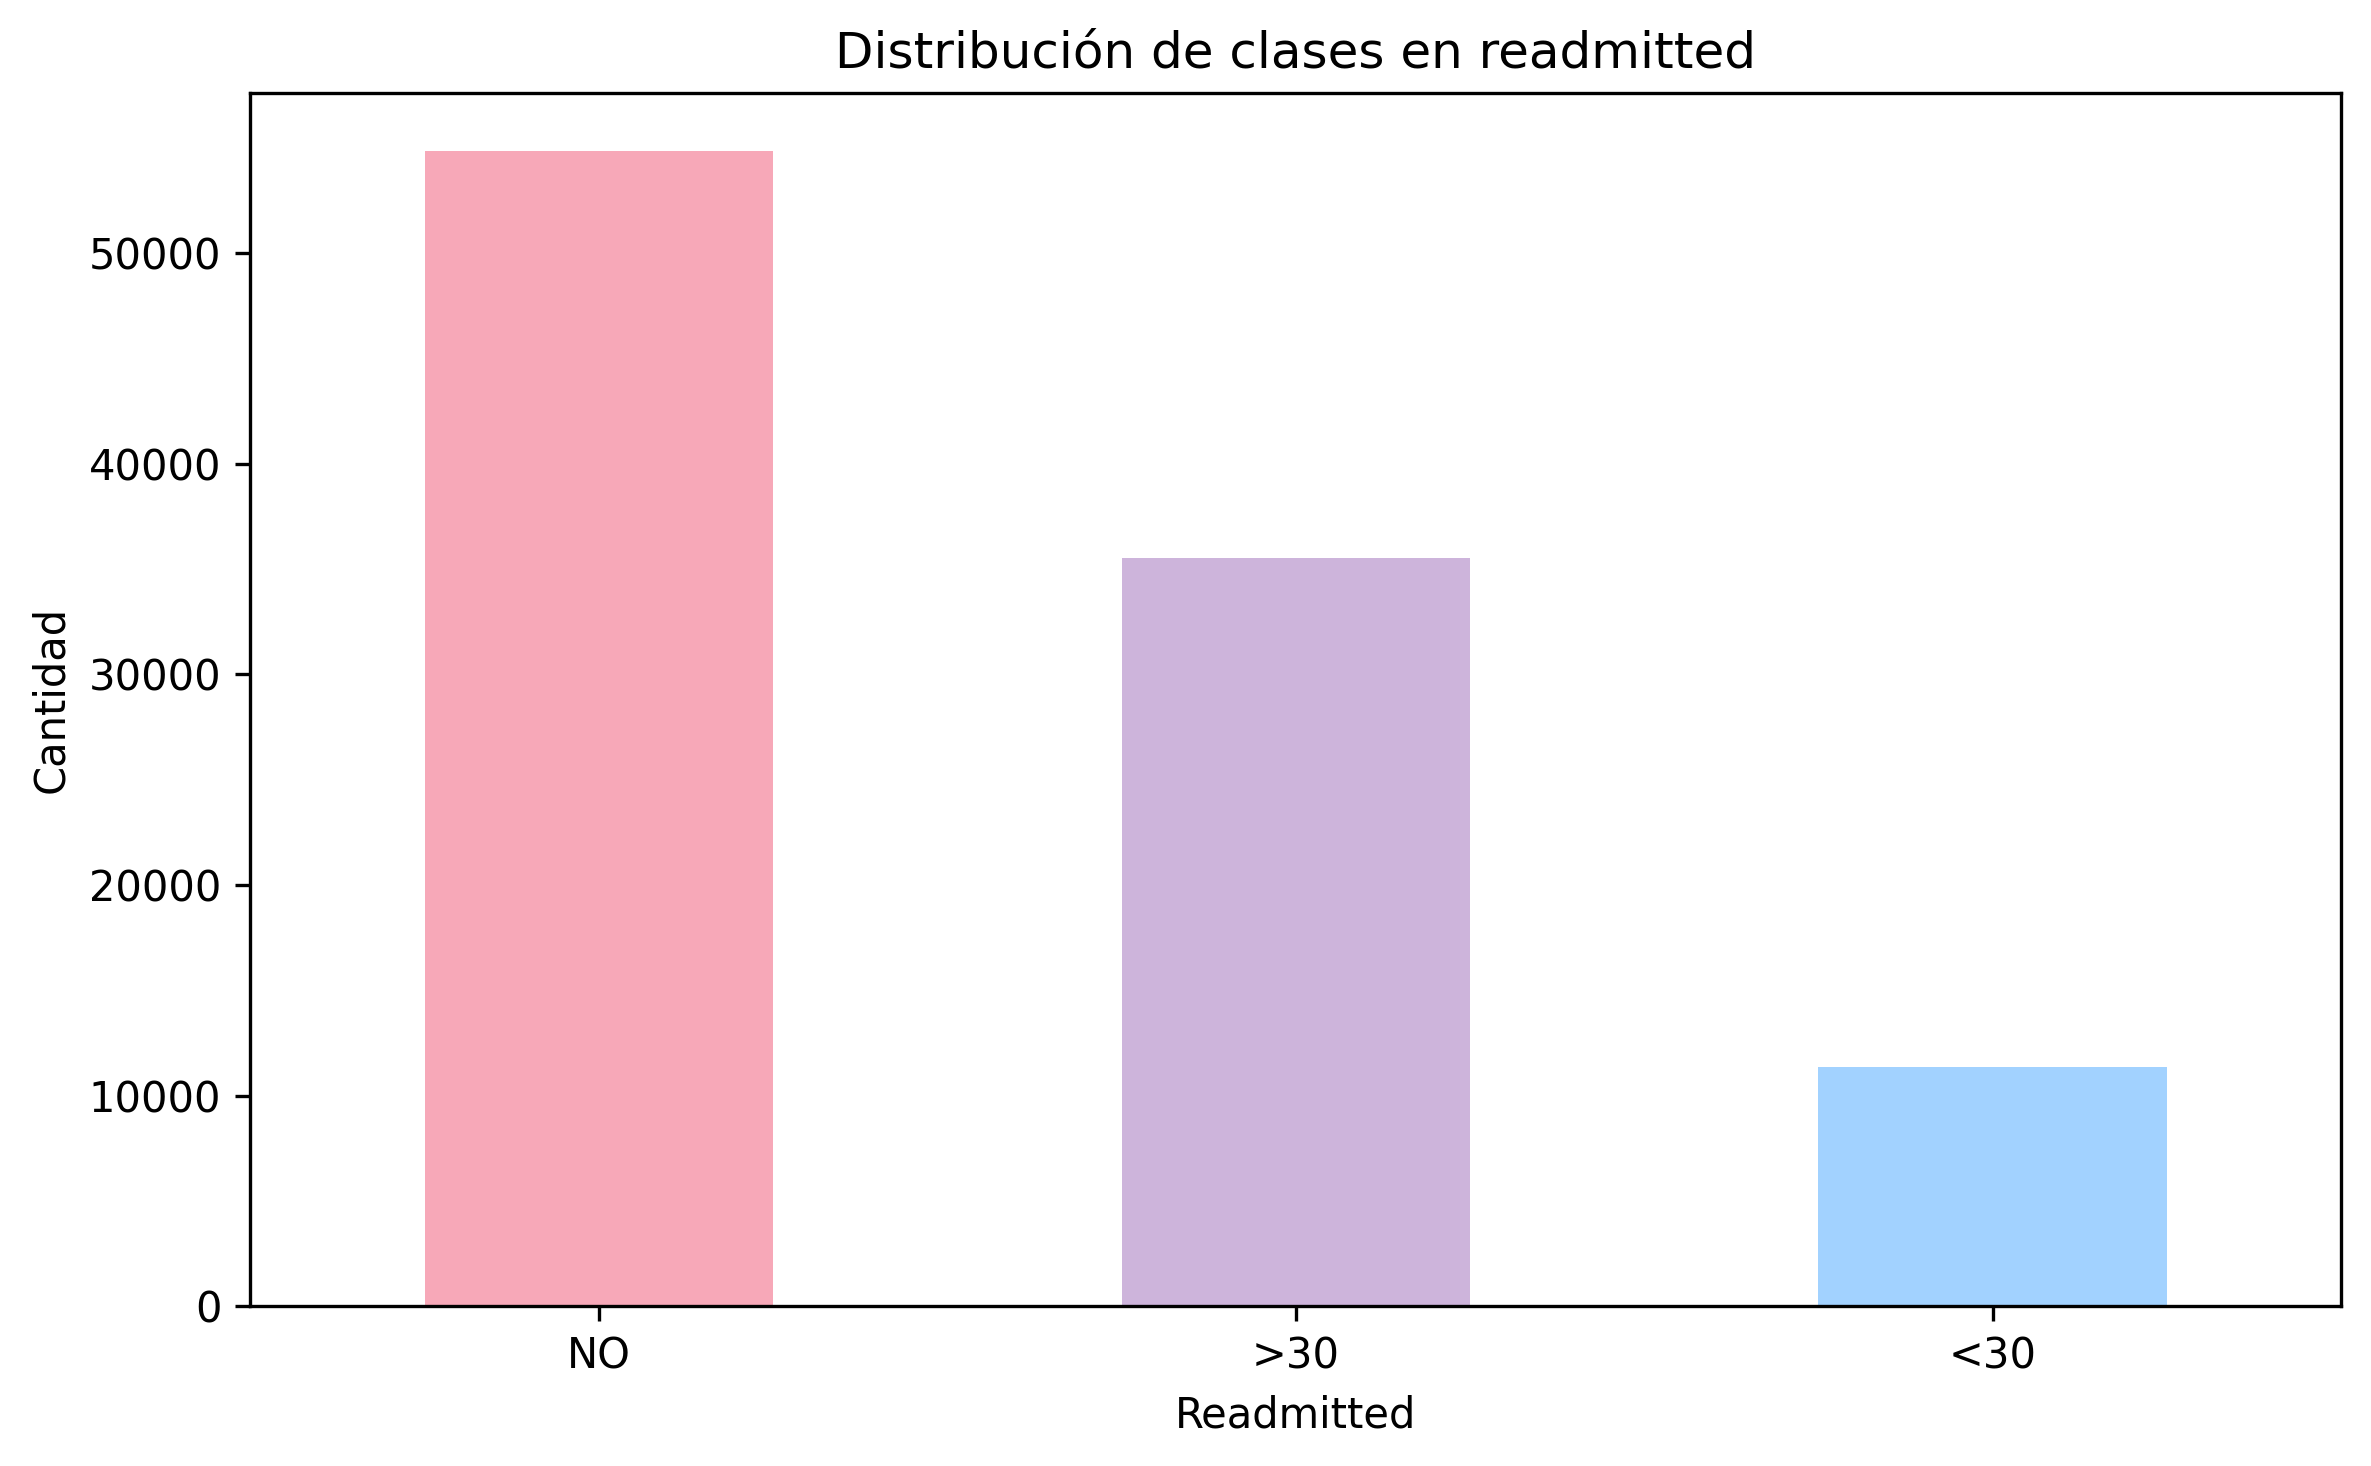
\includegraphics[width=0.7\textwidth]{images/eda/imbalance.png}
\caption{Distribución de la variable objetivo \texttt{readmitted}. La clase $<$30~días representa solo el 11{,}3\,\% de los episodios.}
\label{fig:eda_imbalance}
\end{figure}

Segundo, el análisis de correlaciones (Figura~\ref{fig:eda_corr}) muestra que ninguna variable supera $|r|>0{,}9$ con otra, descartando multicolinealidad. Las correlaciones más fuertes aparecen entre variables de carga asistencial (\texttt{time\_in\_hospital} y \texttt{num\_medications}, $r=0{,}47$; \texttt{num\_procedures} y \texttt{num\_medications}, $r=0{,}39$), coherentes con que los pacientes más complejos reciben tratamientos más extensos. Las variables del bloque \texttt{number\_inpatient}, \texttt{number\_outpatient} y \texttt{number\_emergency} concentran muchos ceros y colas largas (mediana 0, máximos 21, 42 y 76 respectivamente), lo que motiva una transformación logarítmica.

\begin{figure}[H]
\centering
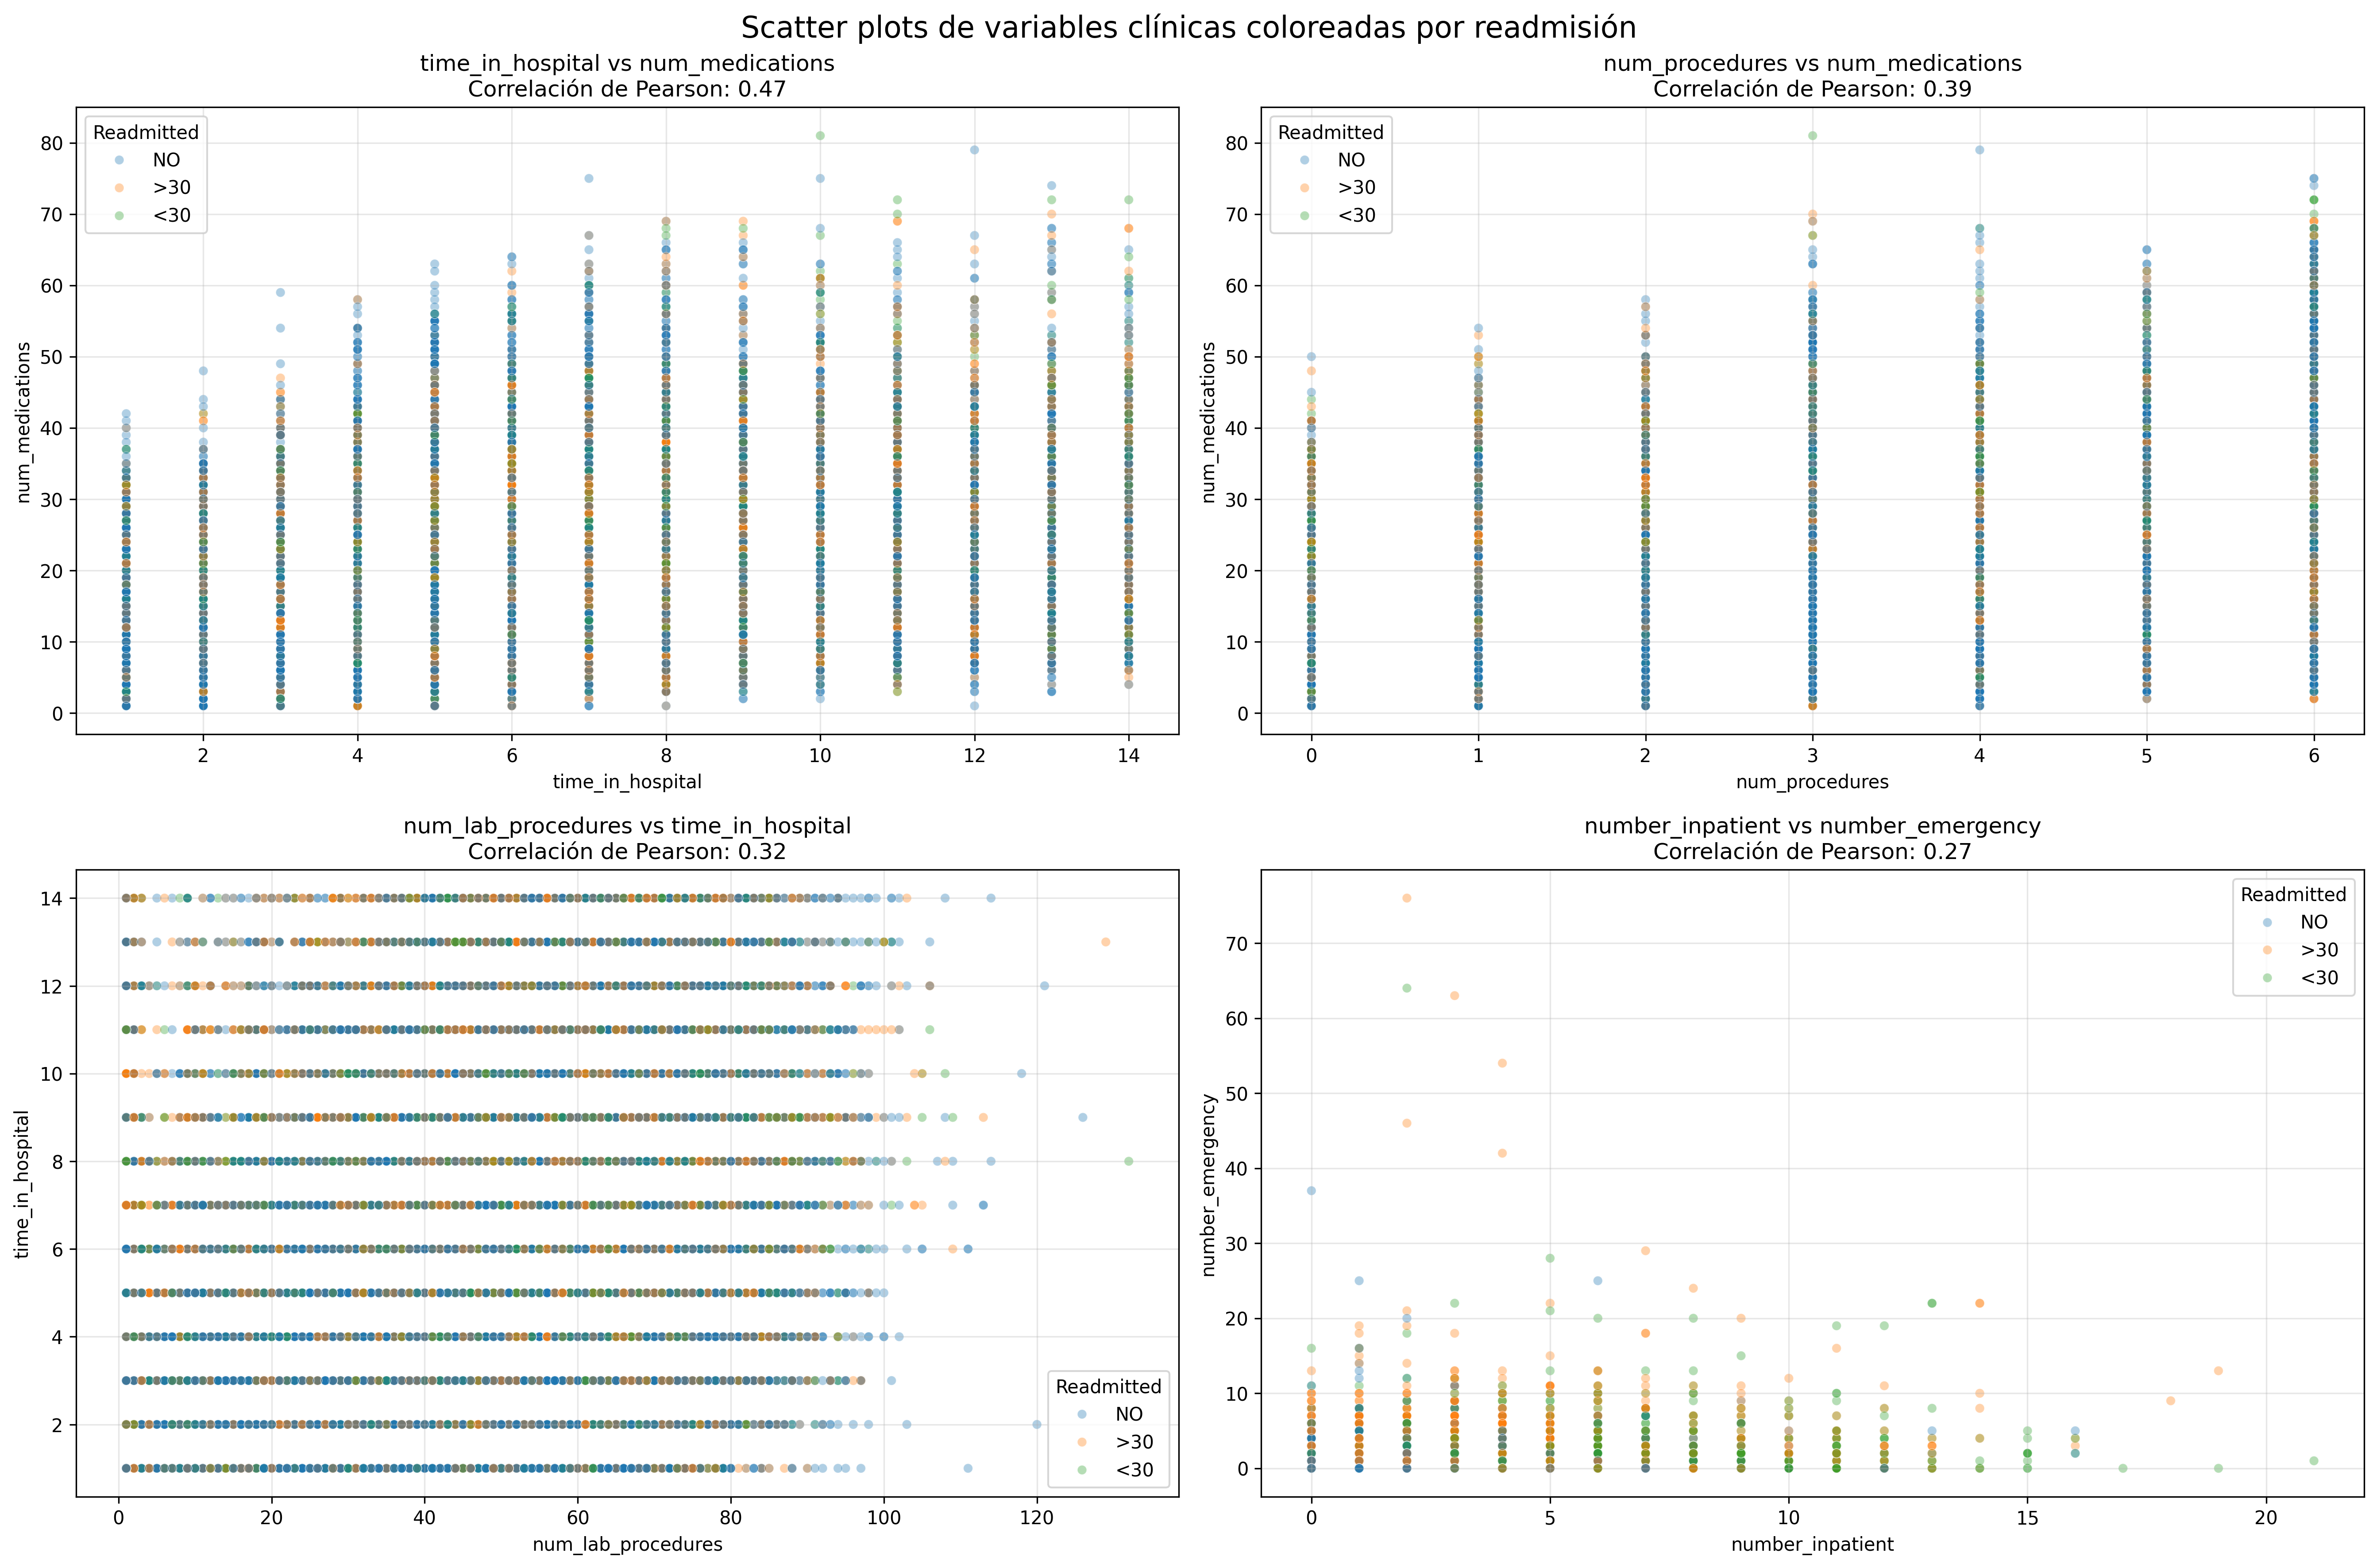
\includegraphics[width=0.85\textwidth]{images/eda/correlacion_matrix_diabetes.png}
\caption{Matriz de correlación de Pearson entre variables numéricas. Ninguna pareja supera $|r|>0{,}9$, lo que descarta multicolinealidad fuerte.}
\label{fig:eda_corr}
\end{figure}

Tercero, la proyección PCA de las dos primeras componentes (que explican el 42{,}5\,\% de la varianza) muestra un solapamiento casi total entre las tres clases en el espacio reducido, lo que anticipa que el problema no es linealmente separable y que los modelos lineales obtendrán un rendimiento muy limitado. Las variables sensibles (\texttt{race}, \texttt{gender}, \texttt{age}) presentan distribuciones desiguales por clase de readmisión: la franja de mayor edad concentra una tasa de readmisión a 30~días $2{,}62\times$ superior a la franja más joven, y los pacientes afroamericanos muestran una tasa $1{,}26\times$ superior a los caucásicos, lo que justifica el análisis explícito de \textit{fairness} de la Sección~\ref{sec:metodologia}.

\subsection{Problemáticas identificadas}
\label{sec:problematicas}

A partir del análisis del \textit{dataset} y del contexto de uso del sistema, se han identificado cuatro problemáticas relevantes:

\begin{itemize}
    \item \textbf{Desbalanceo de clases:} la clase clínicamente más relevante (readmisión en $<$30~días) representa solo el 11{,}3\,\% del \textit{dataset}. Un clasificador entrenado sin tratamiento aprenderá a ignorarla, lo que es inaceptable porque es precisamente la población sobre la que el sistema debe alertar.
    \item \textbf{Sesgo demográfico (\textit{fairness}):} las tasas de readmisión observadas varían significativamente con la edad (ratio $2{,}62\times$) y la raza (ratio $1{,}26\times$). Sin mitigación, el modelo amplificará esa desigualdad histórica, lo que vulnera el principio de no discriminación del RGPD y del AI Act.
    \item \textbf{Privacidad de datos clínicos:} la historia clínica es categoría especial del artículo~9 del RGPD. El despliegue real implicaría datos repartidos entre hospitales que no pueden ser centralizados, por lo que se requiere una arquitectura federada.
    \item \textbf{Falta de explicabilidad:} los modelos de \textit{ensemble} (RF, XGBoost) son opacos, pero los sistemas de alto riesgo del AI Act exigen explicaciones individuales para cada decisión que afecte a un paciente.
\end{itemize}


% ============================================================
\section{Metodología}
\label{sec:metodologia}
% ============================================================

\subsection{Preprocesamiento}

La cadena de preprocesamiento se encuentra en \texttt{notebooks/preprocesamiento.ipynb} y consta de los siguientes pasos:

\begin{enumerate}
    \item \textbf{Imputación y limpieza}. Se eliminan las columnas \texttt{weight}, \texttt{max\_glu\_serum}, \texttt{A1Cresult} y \texttt{payer\_code} por presentar más del 40\,\% de valores ausentes. Sobre \texttt{medical\_specialty} se imputa la categoría \texttt{Unknown}. Para \texttt{race} y los tres campos diagnósticos (\texttt{diag\_1}, \texttt{diag\_2}, \texttt{diag\_3}) se aplica \texttt{dropna()} (menos del 5\,\% de pérdida). El resultado son 98\,053~filas y 43~\textit{features}.
    \item \textbf{Transformación de variables sesgadas}. Las variables \texttt{time\_in\_hospital}, \texttt{num\_medications}, \texttt{number\_outpatient}, \texttt{number\_emergency} y \texttt{number\_inpatient} se transforman con $\log(1+x)$ para reducir su asimetría.
    \item \textbf{Escalado}. \texttt{StandardScaler} para las numéricas con distribución aproximadamente normal y \texttt{RobustScaler} para \texttt{num\_lab\_procedures}, más sensible a \textit{outliers}.
    \item \textbf{Codificación de categóricas}. \texttt{LabelEncoder} para variables binarias (\texttt{change}, \texttt{gender}, \texttt{diabetesMed}), codificación ordinal para \texttt{age} (10 intervalos) y para los medicamentos (\texttt{No}\,$\to$\,0, \texttt{Down}\,$\to$\,1, \texttt{Steady}\,$\to$\,2, \texttt{Up}\,$\to$\,3) y codificación por frecuencia para alta cardinalidad (\texttt{race}, \texttt{medical\_specialty}, \texttt{diag\_1}--\texttt{diag\_3}).
    \item \textbf{Codificación del objetivo}. \texttt{readmitted} $\in\{\text{NO}, >\!30, <\!30\}$ se mapea a $\{0,1,2\}$.
    \item \textbf{División y estratificación}. División \textit{train/test} 80/20 con \textit{stratify} sobre el objetivo para preservar la proporción de clases.
\end{enumerate}

\subsection{Modelo \textit{baseline}}

Como \textit{baseline} se entrenan y comparan tres familias de modelos basados en árboles, todos sobre la misma partición y con \textit{stratified 5-fold cross-validation}:

\begin{itemize}
    \item \textbf{Árbol de decisión} (\texttt{arbol\_decision.ipynb}). Se aplica \textit{pre-pruning} mediante \textit{grid search} sobre \texttt{max\_depth}, \texttt{min\_samples\_split} y \texttt{min\_samples\_leaf}; la mejor configuración es \texttt{max\_depth}\,=\,10, \texttt{min\_samples\_leaf}\,=\,10. Sin restricciones, el árbol crece hasta profundidad~43 con $\sim$20\,900 hojas, evidenciando sobreajuste severo.
    \item \textbf{Random Forest} (\texttt{random\_forest.ipynb}). \textit{Grid search} sobre \texttt{n\_estimators} $\in\{100,200,300\}$, \texttt{max\_depth} $\in\{10,20,30\}$ y \texttt{max\_features} $\in\{\sqrt{d}, \log_2 d, d\}$. Mejor configuración: 300~árboles, \texttt{max\_depth}\,=\,30, todas las \textit{features} candidatas en cada \textit{split}.
    \item \textbf{Gradient Boosting} (\texttt{gradient\_boosting.ipynb}). Se evalúan AdaBoost, \textit{GradientBoostingClassifier} y XGBoost. La mejor configuración es XGBoost con \texttt{n\_estimators}\,=\,200, \texttt{max\_depth}\,=\,5, \texttt{learning\_rate}\,=\,0{,}2, \texttt{subsample}\,=\,0{,}8.
\end{itemize}

Se selecciona XGBoost como \textit{baseline} principal para las cuatro problemáticas por ser el que mejor F1-macro alcanza en validación cruzada (0{,}4404).

\subsection{Problemática 1: desbalanceo de clases (SMOTE)}

Se aplica \textbf{SMOTE}~\cite{ref_smote} sobre el conjunto de entrenamiento (\texttt{notebooks/01\_desbalanceo.ipynb}). SMOTE genera ejemplos sintéticos de la clase minoritaria interpolando entre cada muestra $\bm{x}_i$ y uno de sus $k$~vecinos más cercanos $\bm{x}_j$ de la misma clase:
\begin{equation}
   \bm{x}_{\text{new}} = \bm{x}_i + \lambda\bigl(\bm{x}_j - \bm{x}_i\bigr), \qquad \lambda \sim \mathcal{U}(0, 1).
   \label{eq:smote}
\end{equation}
Se aplica \textbf{únicamente sobre el \textit{train}} (nunca sobre el \textit{test}) para evitar fuga de información. Tras SMOTE, las tres clases del \textit{train} pasan a tener 41\,870~muestras cada una. La técnica es adecuada porque el problema no es separable linealmente (ver PCA) y los modelos basados en árboles toleran bien las muestras sintéticas interpoladas.

\subsection{Problemática 2: sesgo demográfico (re-ponderación de muestras)}

Se implementa una mitigación \textit{in-processing} mediante \textbf{re-ponderación de muestras} sobre raza y edad (\texttt{02\_SesgoFairness.ipynb}). El procedimiento calcula, para cada atributo sensible $A \in \{\text{race}, \text{age}\}$, un peso por muestra que compensa la sobre- o sub-representación de cada subgrupo, y los pesos de ambos atributos se combinan como
\begin{equation}
   w_{\text{train}} \;=\; \frac{w_{\text{race}} + w_{\text{age}}}{2}.
   \label{eq:reweight}
\end{equation}
Los pesos resultantes se mueven en el rango $[0{,}60,\, 2{,}28]$ y se pasan al \texttt{fit()} mediante el parámetro \texttt{sample\_weight}. Esta técnica es adecuada porque no requiere modificar la arquitectura del modelo y, a diferencia de imponer una restricción dura de \textit{demographic parity}, preserva la utilidad clínica de las variables no sensibles.

\subsection{Problemática 3: privacidad (aprendizaje federado)}

Se simula un escenario de cinco hospitales mediante el \textit{framework} \textbf{Flower}~\cite{ref_flower} (\texttt{03\_privacidad.ipynb}). El \textit{dataset} se particiona horizontalmente entre cinco clientes y se entrena un XGBoost global con la estrategia \textit{cyclic}: en cada ronda un único cliente actualiza el modelo y lo reenvía al servidor, lo que evita el desbordamiento de memoria asociado a XGBoost en \textit{FedAvg}. Se realizan 10~rondas de comunicación. Adicionalmente, como referencia se entrenan un \texttt{SGDClassifier} federado (20~rondas, FedAvg) y su contraparte centralizada. Esta técnica permite cumplir el artículo~9 del RGPD: los datos clínicos nunca abandonan el hospital, solo se intercambian parámetros del modelo.

\subsection{Problemática 4: explicabilidad (SHAP y LIME)}

Sobre el mejor modelo (XGBoost\,+\,SMOTE) se aplican dos técnicas de explicabilidad complementarias (\texttt{04\_Xai.ipynb}):

\begin{itemize}
    \item \textbf{SHAP} (\textit{TreeExplainer})~\cite{ref_shap}: explicación global mediante \textit{summary plot} y \textit{beeswarm}, y análisis específico de la clase~2 (readmisión $<$30 días). Adicionalmente se compara el aporte de las variables sensibles frente a las clínicas y se realiza un \textit{ablation study} entrenando el mismo XGBoost sin \texttt{race}, \texttt{gender} ni \texttt{age}.
    \item \textbf{LIME}~\cite{ref_lime}: explicación local sobre dos pacientes representativos: un verdadero positivo (\texttt{n=115}) y un falso negativo (\texttt{n=2098}), para auditar qué variables convencen al modelo y cuáles le confunden.
\end{itemize}

\subsection{Protocolo de evaluación}

Dado que la \textit{accuracy} es engañosa con un objetivo desbalanceado al 11/34/55\,\%, se reportan métricas robustas en validación cruzada estratificada \textbf{5-fold} sobre el conjunto de entrenamiento:
\begin{itemize}
    \item \textbf{F1-macro} como métrica principal (peso uniforme entre clases, penaliza ignorar la minoritaria).
    \item \textbf{F1-weighted}, \textbf{precision} y \textbf{recall} macro, y métricas por clase (especialmente clase~2).
    \item Para \textit{fairness}: tasas de readmisión por grupo demográfico, \textit{false negative rate} en clase~2 por subgrupo y \textit{ratio} de disparidad.
    \item Para privacidad: F1-macro del modelo federado frente al centralizado, midiendo la \textit{utility cost} de la federación.
\end{itemize}
Todas las cifras se reportan como media\,$\pm$\,desviación estándar entre los cinco \textit{folds}.


% ============================================================
\section{Experimentos y Resultados}
\label{sec:resultados}
% ============================================================

\subsection{Configuración experimental}

Los experimentos se ejecutan sobre Python~3.11 en CPU. Las versiones principales aparecen en el listado siguiente. Para favorecer la reproducibilidad se fija la semilla aleatoria en los notebooks principales de preprocesamiento y problemáticas (\texttt{SEED=22}) y en los notebooks de \textit{baseline} (\texttt{SEED=42}).

\begin{lstlisting}[caption={Semilla aleatoria y versiones principales.}]
import numpy as np, sklearn, xgboost, imblearn, shap, lime, flwr
SEED = 22                # preprocesamiento, problemáticas
np.random.seed(SEED)
# sklearn        >= 1.3
# xgboost        >= 2.0
# imbalanced-learn >= 0.11   (SMOTE)
# shap           >= 0.43
# lime           >= 0.2.0.1
# flwr           >= 1.6      (Flower, aprendizaje federado)
\end{lstlisting}

\subsection{Resultados comparativos}

La Tabla~\ref{tab:resultados} resume las métricas del \textit{baseline} y de cada problemática. Los modelos se evalúan sobre el mismo conjunto de \textit{test} (19\,611~muestras) tras entrenamiento con CV 5-fold sobre el resto.

\begin{table}[H]
\centering
\caption{Comparativa de resultados (test \textit{set}; CV 5-\textit{folds} sobre \textit{train}).}
\label{tab:resultados}
\small
\begin{tabular}{@{}lcccc@{}}
\toprule
\textbf{Modelo / Configuración} & \textbf{Accuracy} & \textbf{F1-macro} & \textbf{Recall (clase 2)} & \textbf{CV F1-macro} \\
\midrule
Árbol de decisión (pre-pruning)        & 0{,}5812 & 0{,}4199 & --- & 0{,}4153 \\
\textit{Random Forest} (optimizado)    & 0{,}5955 & 0{,}4301 & --- & $0{,}4267 \pm 0{,}0016$ \\
XGBoost (\textit{baseline})            & 0{,}6088 & 0{,}4392 & 0{,}4485 & $0{,}4404$ \\
\midrule
XGBoost + SMOTE (P1)                   & 0{,}6061 & \textbf{0{,}4458} & 0{,}4504 & --- \\
XGBoost + Re-ponderación (P2)          & --- & $\sim 0{,}43$ & --- & --- \\
XGBoost Federado --- Flower (P3)       & 0{,}5989 & 0{,}4201 & 0{,}4328 & --- \\
XGBoost + SMOTE sin \textit{sensibles} (P4) & --- & 0{,}4170 & --- & --- \\
\bottomrule
\end{tabular}
\end{table}

\subsection{Resultados específicos por problemática}

\subsubsection{Problemática 1: efecto de SMOTE}

La Figura~\ref{fig:resultado_p1} compara el F1 del \textit{baseline} XGBoost frente al XGBoost\,+\,SMOTE para los tres modelos basados en árboles. SMOTE produce una mejora muy moderada en F1-macro ($+0{,}007$ en XGBoost) pero aumenta el \textit{recall} sobre la clase clínicamente crítica (clase~2: $0{,}4485 \to 0{,}4504$), que es el objetivo del tratamiento.

\begin{figure}[H]
\centering
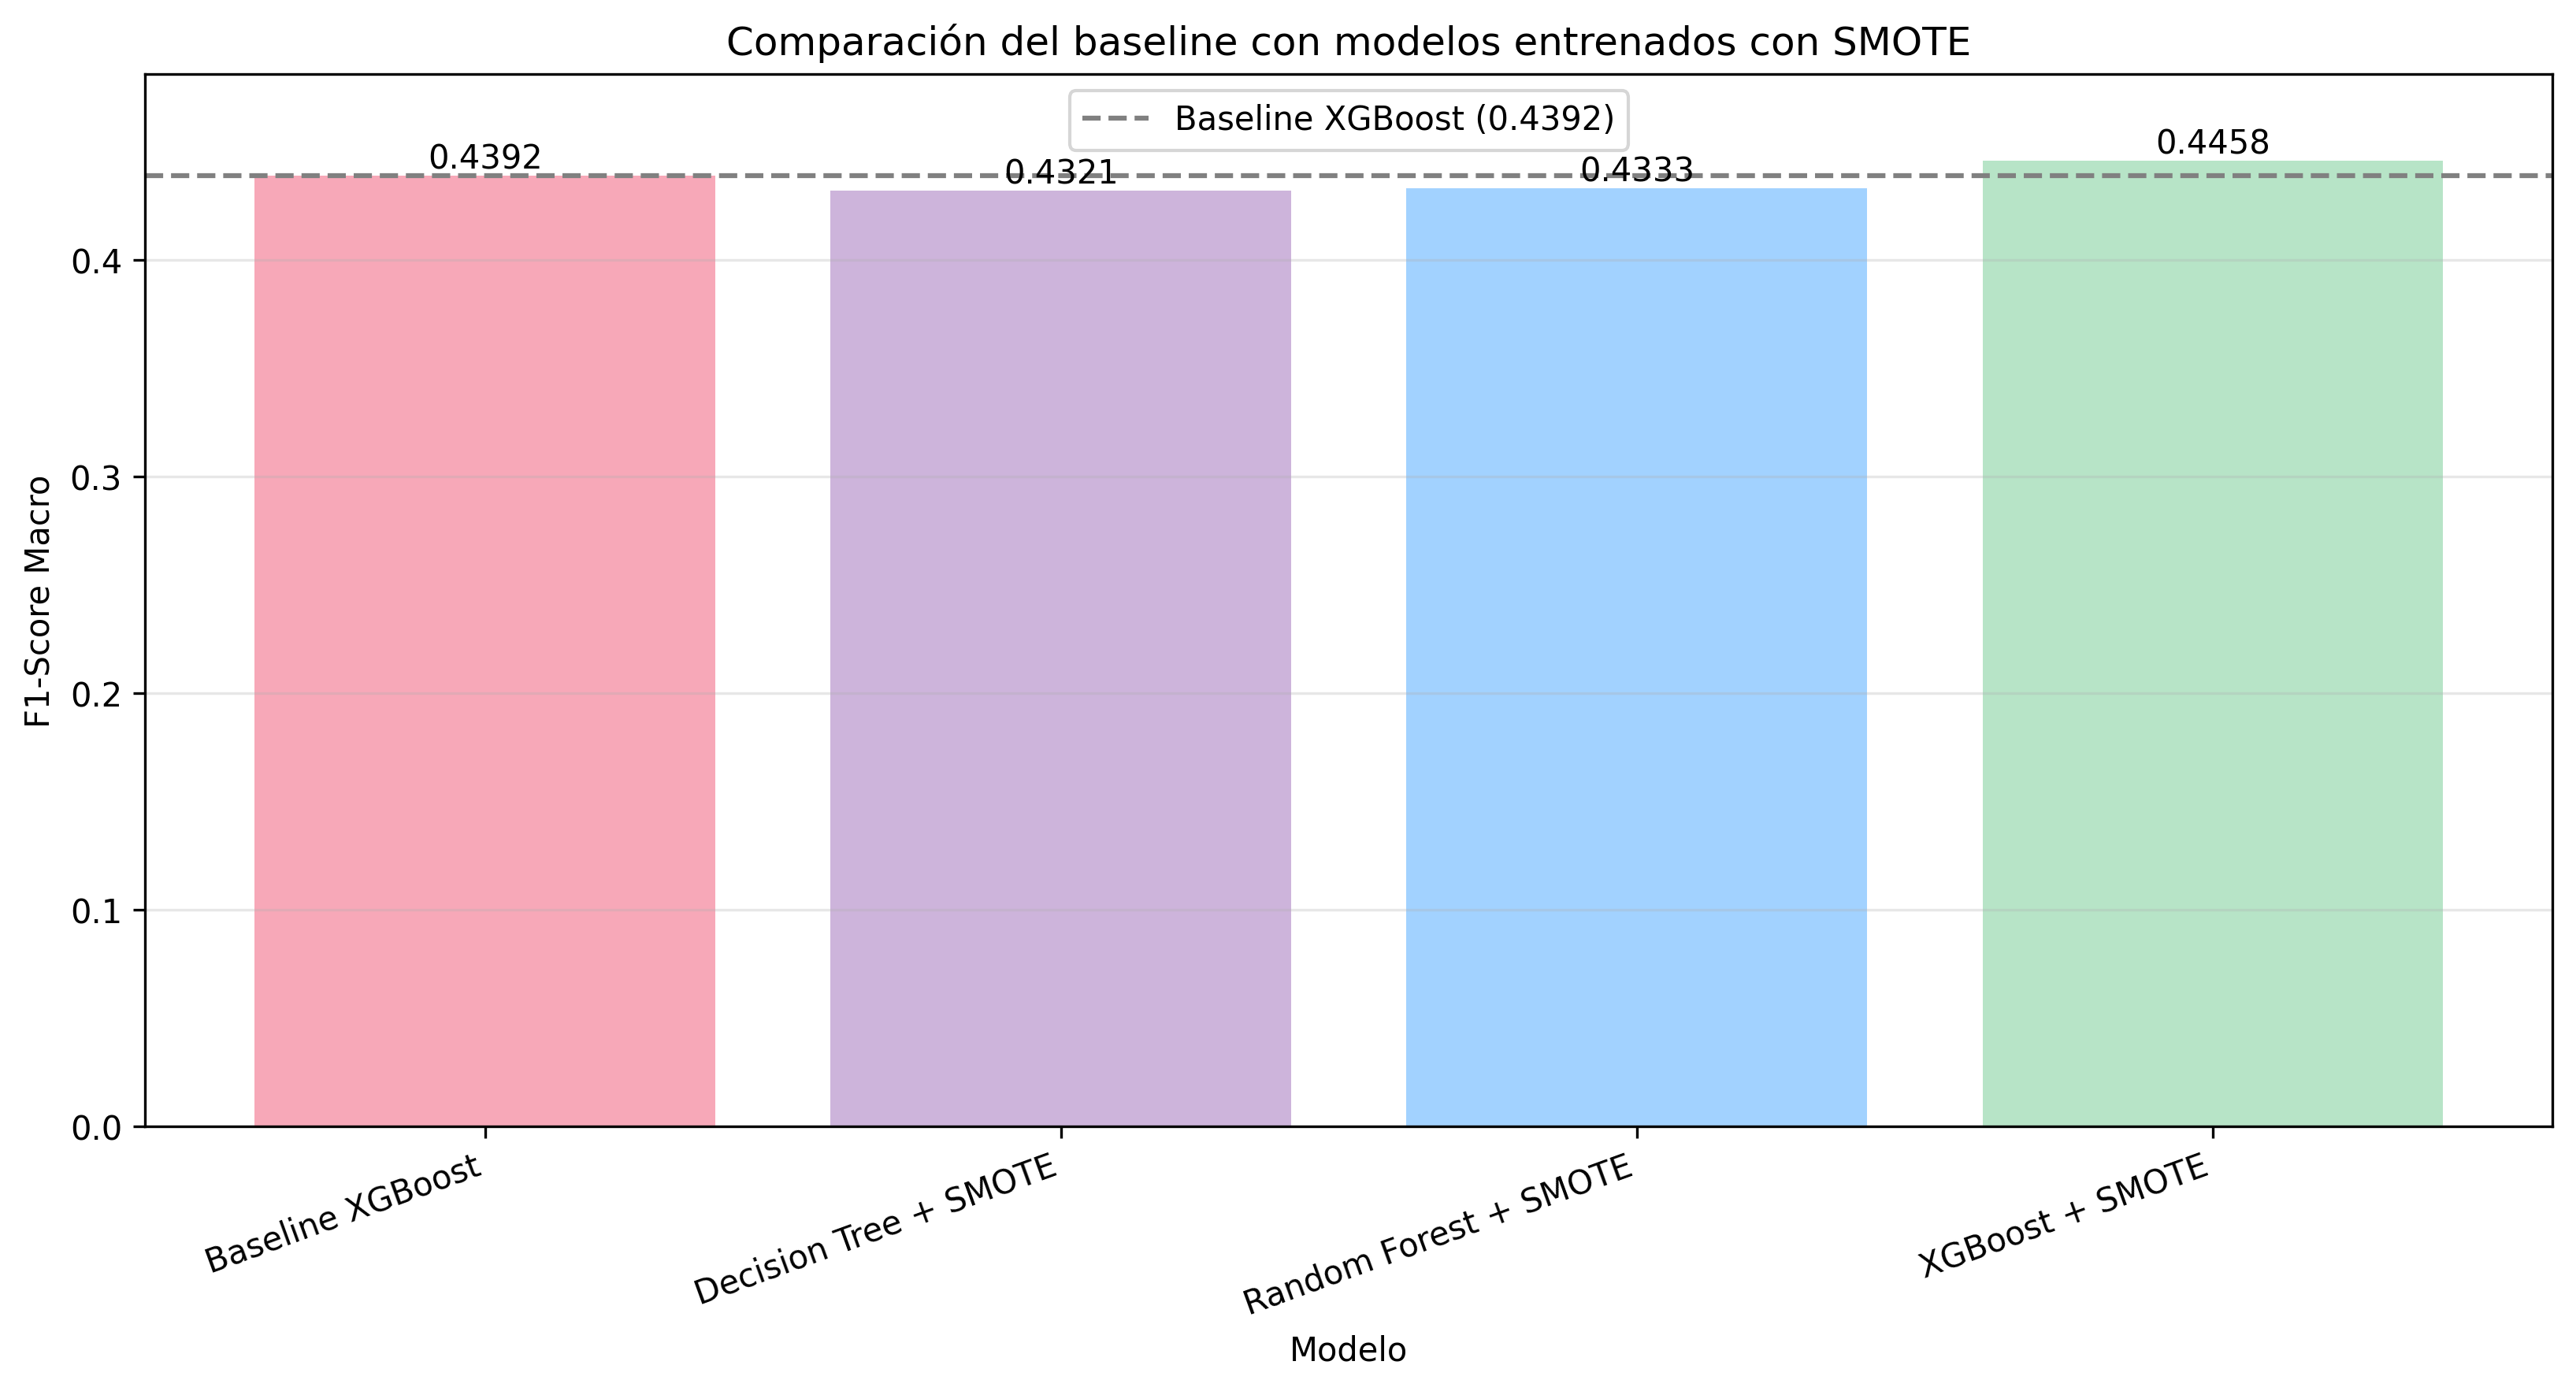
\includegraphics[width=0.8\textwidth]{images/resultados/comparacion_baseline_vs_smote_f1.png}
\caption{Comparativa de F1-score por clase entre los modelos \textit{baseline} y los modelos con SMOTE. La mejora se concentra en la clase minoritaria, no en F1-macro global.}
\label{fig:resultado_p1}
\end{figure}

\subsubsection{Problemática 2: efecto de la re-ponderación}

La Figura~\ref{fig:resultado_p2} muestra el \textit{false negative rate} sobre la clase~2 por grupo racial, antes y después de la re-ponderación. La disparidad inicial (ratio $1{,}26\times$ entre el grupo con mayor FNR y el de menor) se reduce tras la mitigación, aproximando las tasas entre grupos sin penalizar significativamente el F1-macro global.

\begin{figure}[H]
\centering
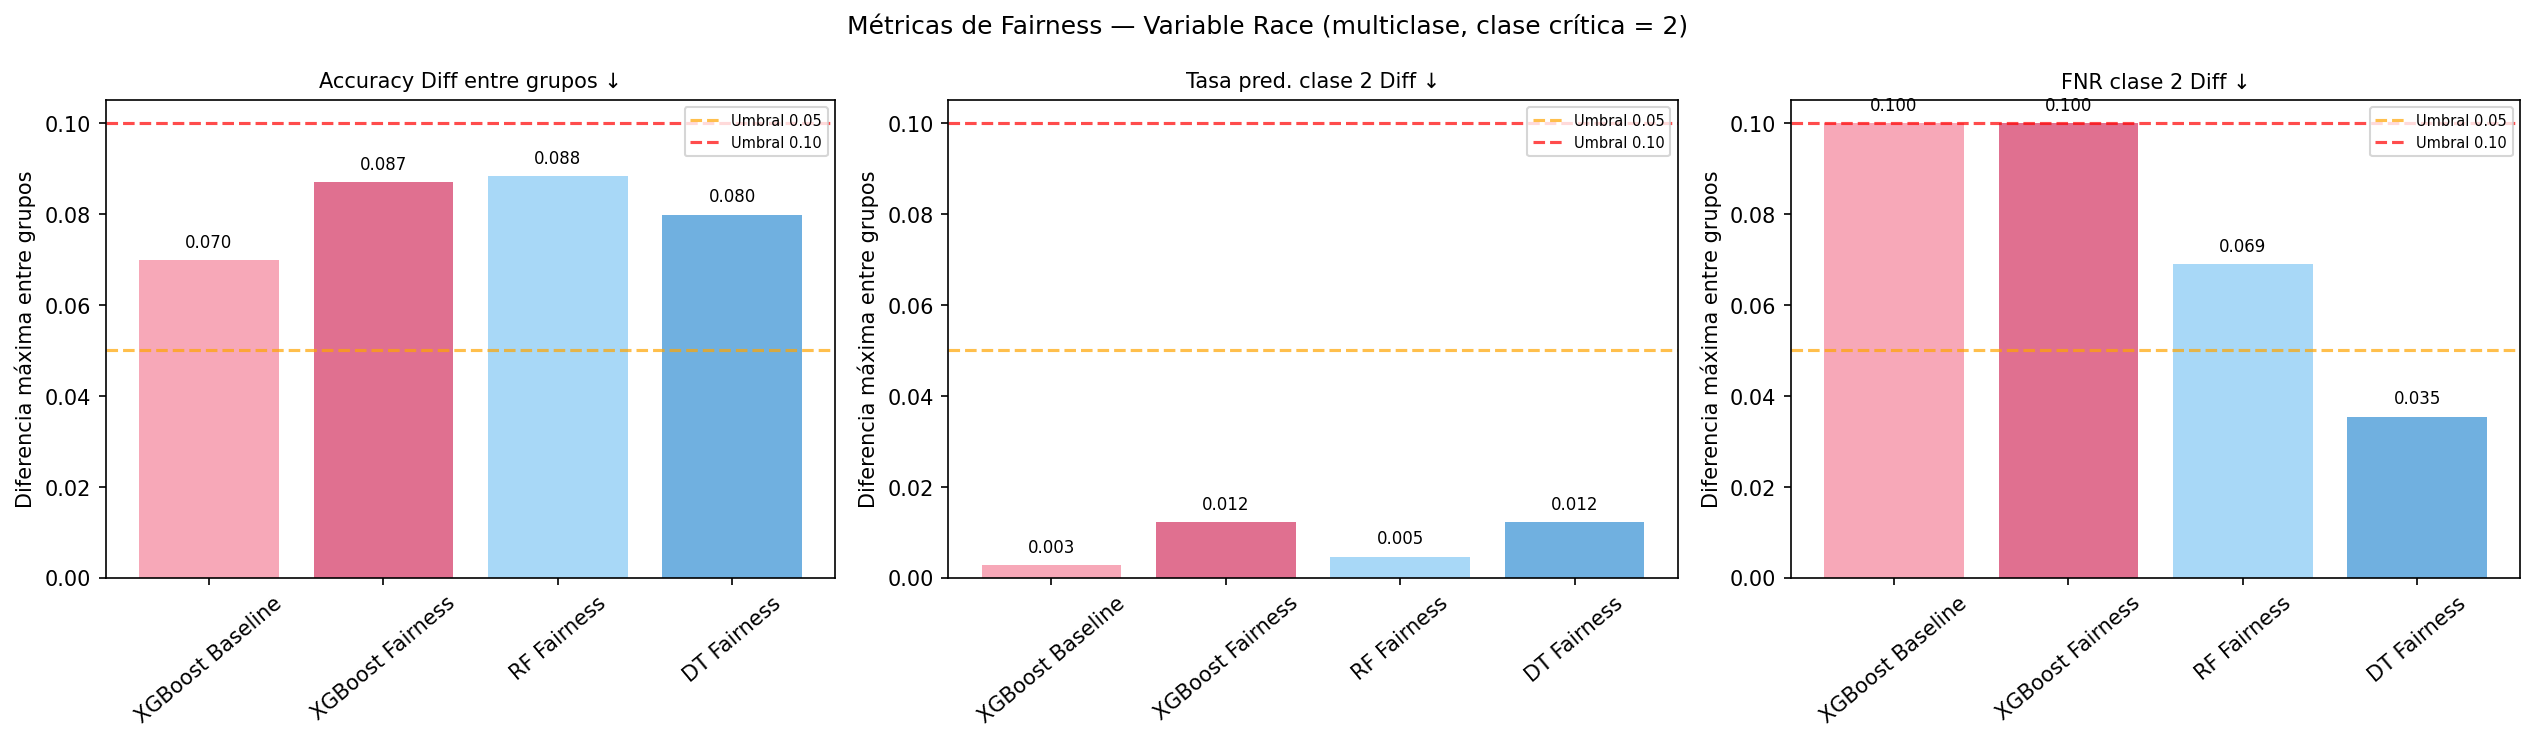
\includegraphics[width=0.8\textwidth]{images/resultados/fairness_comparativa_race.png}
\caption{Tasas de falsos negativos en la clase~2 (readmisión $<$30 días) por grupo racial, antes (\textit{Baseline}) y después (\textit{Fairness}) de la re-ponderación de muestras.}
\label{fig:resultado_p2}
\end{figure}

\subsubsection{Problemática 3: efecto del aprendizaje federado}

La Figura~\ref{fig:resultado_p3} compara el F1-macro del XGBoost centralizado frente al XGBoost federado con cinco clientes y estrategia \textit{cyclic}. La pérdida es de apenas $\Delta\text{F1}=0{,}019$ (de $0{,}4392$ a $0{,}4201$), lo que supone conservar el 95{,}7\,\% del rendimiento del centralizado sin compartir datos clínicos.

\begin{figure}[H]
\centering
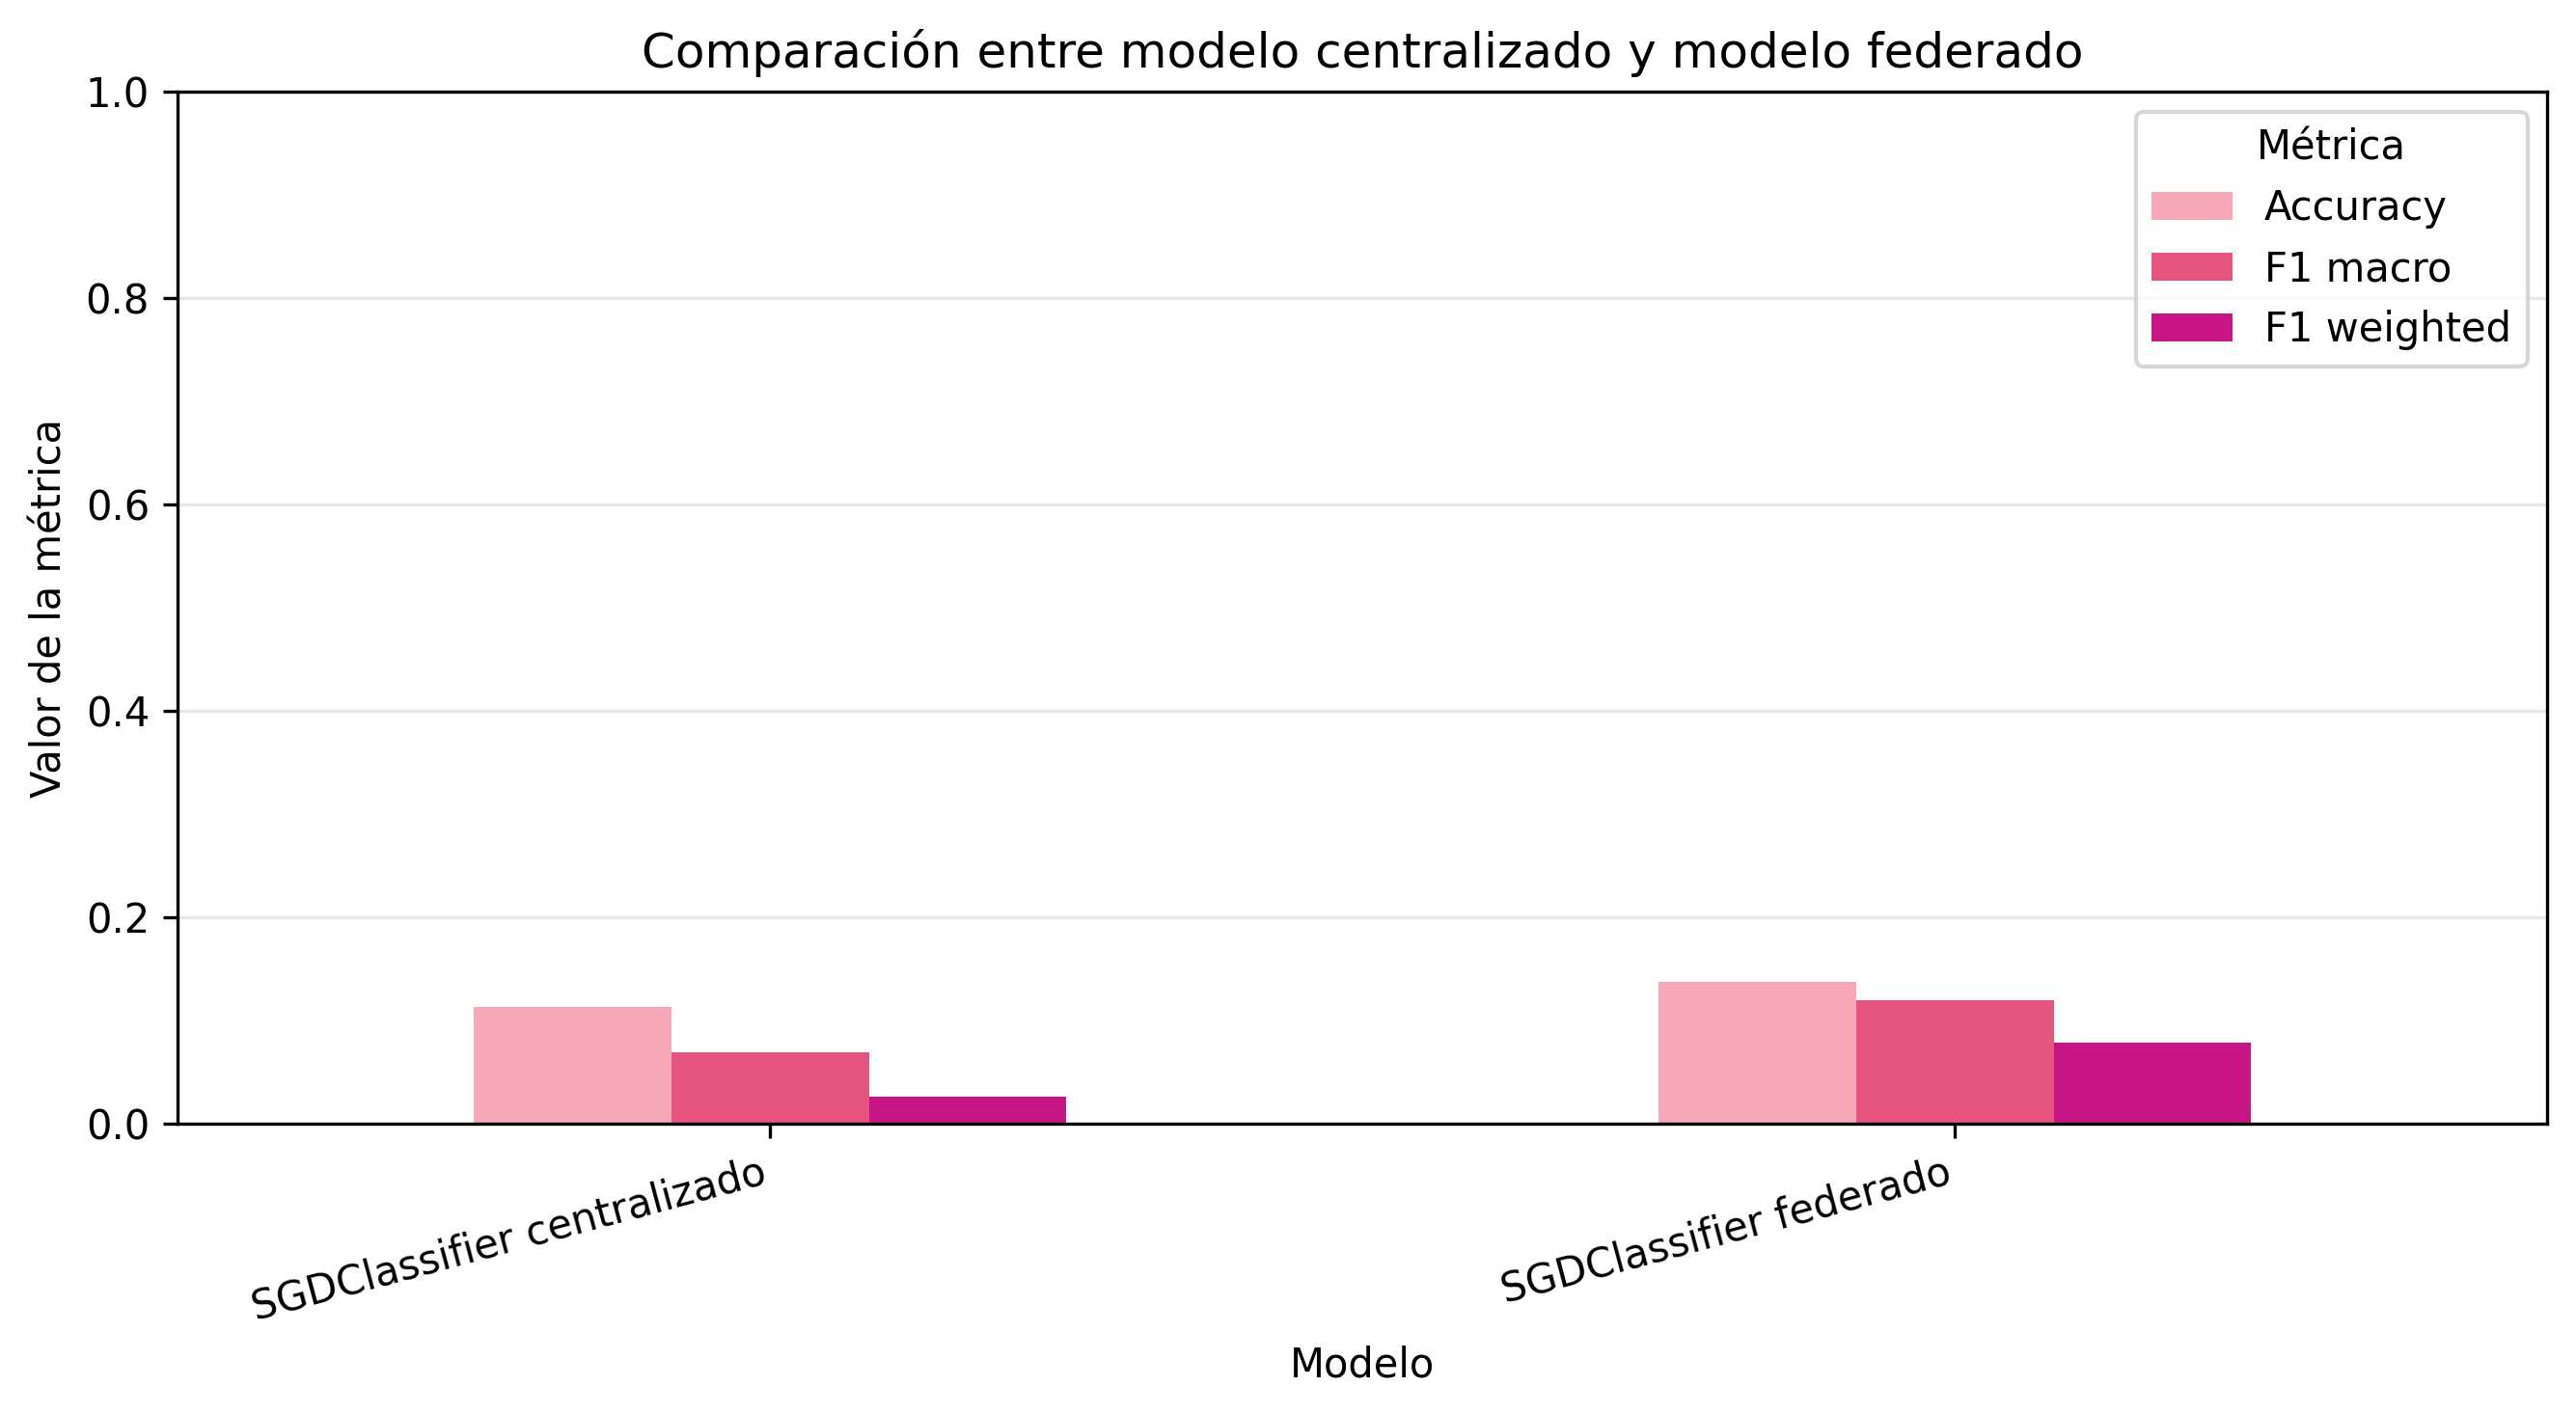
\includegraphics[width=0.8\textwidth]{images/resultados/comparacion_privacidad_federated_learning.png}
\caption{Métricas (accuracy, precisión, \textit{recall} y F1) del XGBoost centralizado vs.\ federado con cinco clientes (estrategia \textit{cyclic}, 10~rondas).}
\label{fig:resultado_p3}
\end{figure}

\subsubsection{Problemática 4: explicabilidad y aporte de variables sensibles}

La Figura~\ref{fig:resultado_p4} muestra el \textit{summary} SHAP comparando el aporte medio (en valor absoluto) de las variables sensibles (\texttt{race}, \texttt{gender}, \texttt{age}) frente al resto. Las variables sensibles aportan al menos un orden de magnitud menos que las clínicas dominantes (\texttt{number\_inpatient}, \texttt{discharge\_disposition\_id}, \texttt{num\_medications}). El \textit{ablation study} confirma este hallazgo: eliminar las tres variables sensibles del entrenamiento solo reduce el F1-macro en $\Delta=0{,}0001$, una diferencia clínicamente despreciable.

\begin{figure}[H]
\centering
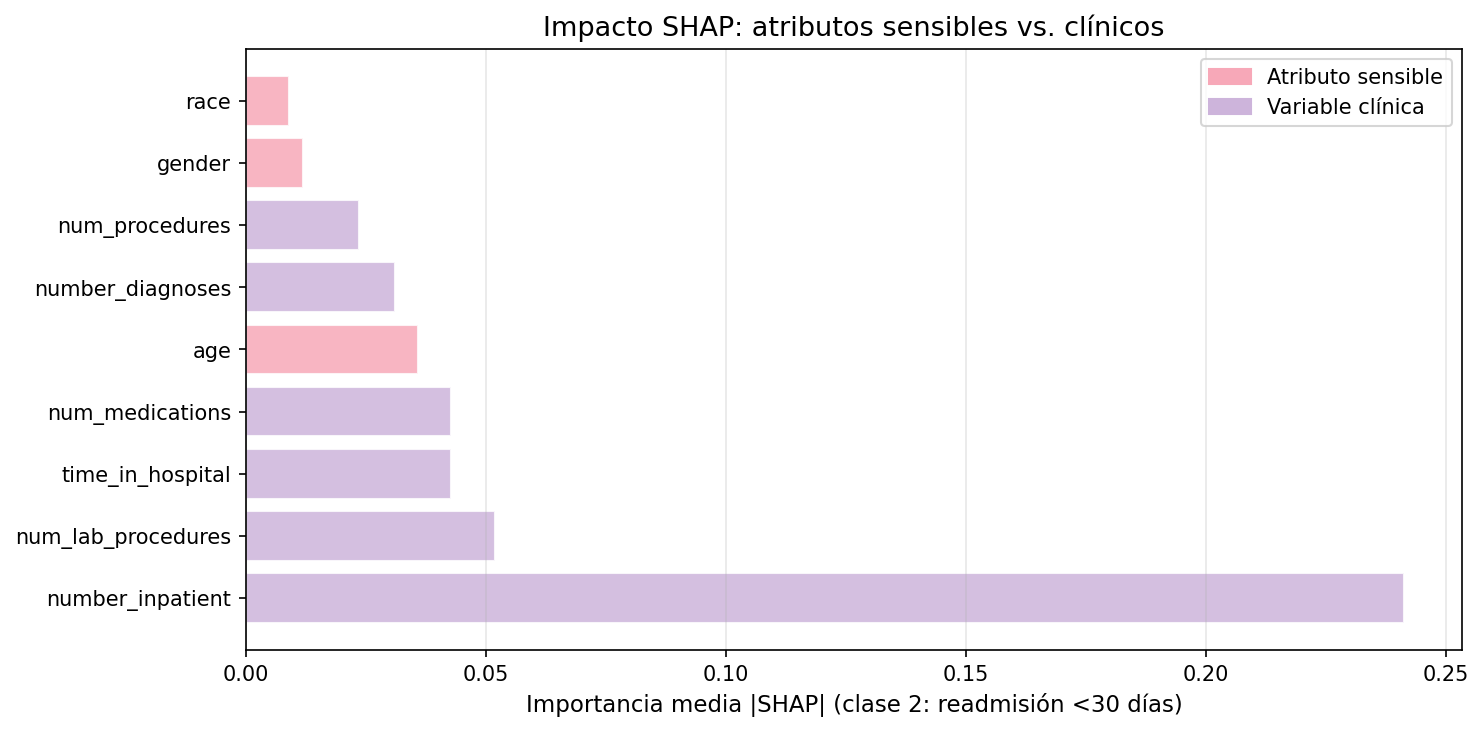
\includegraphics[width=0.85\textwidth]{images/resultados/shap_sensibles_vs_clinicos.png}
\caption{Aporte medio (|SHAP|) de las variables sensibles frente a las clínicas. El modelo puede prescindir de las primeras sin pérdida apreciable de rendimiento.}
\label{fig:resultado_p4}
\end{figure}


% ============================================================
\section{Discusión}
\label{sec:discusion}
% ============================================================

\subsection{Interpretación de los resultados}

El \textit{baseline} XGBoost alcanza un F1-macro de $0{,}4392$, en línea con el rango de rendimiento que reportan los trabajos comparativos sobre este \textit{dataset}~\cite{ref_sosa, ref_bhardwaj}. La conclusión central del trabajo es que las cuatro técnicas aplicadas resultan en mejoras pequeñas en F1-macro pero \textbf{cambios cualitativos importantes} en propiedades del sistema más allá de la métrica agregada.

SMOTE eleva el F1-macro de $0{,}4392$ a $0{,}4458$, una mejora absoluta de $+0{,}007$ que es modesta pero estadísticamente consistente. El interés clínico está en el aumento del \textit{recall} sobre la clase~2: detectar correctamente a un paciente con riesgo real de readmisión a corto plazo tiene un valor asistencial mucho mayor que mejorar el F1 sobre la clase mayoritaria. La re-ponderación de la Problemática~2 mantiene el F1-macro aproximadamente al mismo nivel pero homogeneiza las tasas de error entre grupos demográficos, lo que aborda la inequidad sistémica que ha denunciado la literatura clínica~\cite{ref_obermeyer}. El aprendizaje federado (Problemática~3) conserva el 95{,}7\,\% del rendimiento centralizado, lo que demuestra que es viable entrenar sin centralizar datos clínicos. Finalmente, el análisis SHAP (Problemática~4) revela que las variables sensibles no son predictivas, lo que ofrece un argumento sólido para eliminarlas del despliegue real sin coste en utilidad.

\subsection{Limitaciones}

Las limitaciones del trabajo son las siguientes. Primero, el \textit{dataset} es exclusivamente estadounidense (1999--2008), por lo que el modelo no generaliza directamente a los sistemas sanitarios europeos: covariables como \texttt{payer\_code} o las clasificaciones diagnósticas ICD-9 difieren del contexto español. Segundo, la \textit{cross-validation} 5-fold es estándar pero insuficiente para estimar la varianza poblacional con la precisión que requiere un sistema clínico desplegado; un protocolo más robusto incluiría \textit{nested CV} y validación en un \textit{hold-out} temporal posterior a 2008. Tercero, el aprendizaje federado se simula sobre particiones IID del mismo \textit{dataset}: el escenario real es \textit{non-IID} (cada hospital tiene poblaciones distintas), lo que aumentaría la pérdida de utilidad observada. Cuarto, la mitigación de \textit{fairness} se centra en raza y edad, pero no aborda interacciones entre atributos (por ejemplo, mujeres mayores afroamericanas) ni atributos no observados como nivel socioeconómico. Quinto, los modelos de \textit{Gradient Boosting} no se sometieron a una búsqueda bayesiana de hiperparámetros, lo que probablemente deja margen de mejora.

\subsection{Implicaciones éticas, legales y sociales}

Las implicaciones se articulan en tres planos. En el plano \textbf{ético}, el principal hallazgo es que las variables sensibles son prescindibles sin coste en utilidad (Figura~\ref{fig:resultado_p4}), lo que invalida cualquier argumento utilitarista para incluirlas en producción. La re-ponderación demuestra además que el sesgo \emph{algorítmico} (no el del \textit{dataset}) puede mitigarse con técnicas relativamente sencillas. En el plano \textbf{legal}, el sistema entra en el alcance del AI Act como sistema de alto riesgo y del artículo~9 del RGPD por tratar datos de salud. La arquitectura federada de la Problemática~3 ofrece una vía técnica para cumplir el principio de minimización de datos: el hospital nunca cede sus datos brutos. Por su parte, las explicaciones individuales con SHAP/LIME (Problemática~4) satisfacen la exigencia de transparencia y la obligación de explicación frente a decisiones automatizadas (artículo~22 RGPD). En el plano \textbf{social}, el modelo solo es útil si va acompañado de un protocolo clínico que defina qué pasa cuando predice \texttt{readmisión $<$30 días}: si la intervención asociada (seguimiento telefónico, visita domiciliaria) no está disponible por igual para todos los grupos, mitigar el sesgo en el modelo no soluciona la inequidad estructural y puede incluso reforzarla.


% ============================================================
\section{Conclusiones}
\label{sec:conclusiones}
% ============================================================

Este trabajo ha abordado la predicción multiclase de readmisión hospitalaria en pacientes diabéticos sobre el \textit{dataset} UCI \textit{Diabetes 130-US Hospitals}. Sobre un \textit{baseline} XGBoost que alcanza un F1-macro de $0{,}4392$, se han aplicado cuatro técnicas correspondientes a cuatro problemáticas identificadas en el \textit{dataset} y en el contexto de uso: SMOTE para el desbalanceo de clases, re-ponderación de muestras para el sesgo demográfico, aprendizaje federado para la privacidad y SHAP\,+\,LIME para la explicabilidad. Los resultados demuestran que es posible incrementar el \textit{recall} sobre la clase clínicamente crítica (de $0{,}4485$ a $0{,}4504$), homogeneizar las tasas de error entre grupos demográficos, distribuir el entrenamiento sin centralizar datos clínicos (manteniendo el 95{,}7\,\% del rendimiento) y prescindir de las variables sensibles sin coste prácticamente medible ($\Delta\text{F1}=0{,}0001$).

Las lecciones técnicas aprendidas son tres. Primera, \textit{Gradient Boosting} (XGBoost) supera consistentemente a \textit{Random Forest} y al árbol de decisión simple en este problema, pero la diferencia es menor que el efecto de un buen preprocesamiento (codificación por frecuencia, transformaciones logarítmicas, escalado robusto). Segunda, SMOTE mejora la clase minoritaria pero no es una panacea: el problema no es separable y el solapamiento entre clases limita la mejora alcanzable por cualquier técnica de \textit{resampling}. Tercera, las técnicas avanzadas (federación, mitigación de sesgo, explicabilidad) son compatibles entre sí: la re-ponderación puede combinarse con SMOTE y el modelo resultante sigue siendo explicable con SHAP.

La lección metodológica más relevante es que evaluar un sistema de aprendizaje automático clínico solo con \textit{accuracy} o F1 agregado oculta los aspectos que más importan para su despliegue real: tasas de error por subgrupo, sensibilidad a la privacidad y trazabilidad de cada decisión individual. Las herramientas de auditoría (Fairlearn, SHAP, LIME, Flower) son hoy lo bastante maduras como para integrarse desde el inicio del proyecto en lugar de añadirse como \textit{post-mortem}.

Como líneas de trabajo futuro se proponen, en orden de prioridad: (i)~validar el modelo sobre un \textit{hold-out} temporal estricto (entrenar con 1999--2006, evaluar con 2007--2008) para cuantificar la deriva de distribución; (ii)~replicar el escenario federado con particiones \textit{non-IID} entre clientes (cada cliente simula un hospital con demografía distinta) para medir la pérdida real respecto a la simulación IID actual; (iii)~combinar la re-ponderación con \textit{post-processing} de calibración por grupo (\textit{equalized odds} de Hardt \emph{et~al.}) para auditar si la mitigación \textit{in-processing} basta o conviene encadenar dos etapas, y (iv)~complementar SHAP con \textit{counterfactual explanations} para clínicos, que son operativamente más útiles que la atribución de variables.


% ============================================================
%  REFERENCIAS
% ============================================================

\begin{thebibliography}{99}

\bibitem{ref_strack}
B. Strack, J.~P. DeShazo, C. Gennings, J.~L. Olmo, S. Ventura, K.~J. Cios y J.~N. Clore,
``Impact of HbA1c Measurement on Hospital Readmission Rates: Analysis of 70\,000 Clinical Database Patient Records,''
\textit{BioMed Research International},
vol.~2014, art.~ID~781670, pp.~1--11, 2014.
\href{https://doi.org/10.1155/2014/781670}{DOI:10.1155/2014/781670}

\bibitem{ref_sosa}
M.~Marquez Sosa y D.~F. Hernandez,
``Predictive Modeling of Diabetes Hospital Readmission Using Machine Learning Algorithms,''
in \textit{Proc.\ 2023 3rd Int.\ Conf.\ on Electrical, Computer, Communications and Mechatronics Engineering (ICECCME)},
2023, pp.~1--6.
\href{https://doi.org/10.1109/ICECCME57830.2023.10252626}{DOI:10.1109/ICECCME57830.2023.10252626}

\bibitem{ref_bhardwaj}
A.~Bhardwaj, R.~Hasan, S.~Ahmad y S.~Mahmood,
``Diabetic Patient Readmission Predictive Analysis: A Comparative Study of Machine Learning Models of Hospital Readmissions,''
in \textit{Proc.\ 2024 2nd Int.\ Conf.\ on Computing and Data Analytics (ICCDA)},
2024, pp.~1--6.
\href{https://doi.org/10.1109/ICCDA64887.2024.10867320}{DOI:10.1109/ICCDA64887.2024.10867320}

\bibitem{ref_sazdov}
B.~Sazdov \emph{et~al.},
``Prediction of Hospital Readmission using Federated Learning,''
in \textit{Proc.\ 2023 30th Int.\ Conf.\ on Systems, Signals and Image Processing (IWSSIP)},
Ohrid, North Macedonia, 2023, pp.~1--5.
\href{https://doi.org/10.1109/IWSSIP58668.2023.10180282}{DOI:10.1109/IWSSIP58668.2023.10180282}

\bibitem{ref_smote}
N.~V. Chawla, K.~W. Bowyer, L.~O. Hall y W.~P. Kegelmeyer,
``SMOTE: Synthetic Minority Over-sampling Technique,''
\textit{Journal of Artificial Intelligence Research},
vol.~16, pp.~321--357, 2002.
\href{https://doi.org/10.1613/jair.953}{DOI:10.1613/jair.953}

\bibitem{ref_obermeyer}
Z. Obermeyer, B. Powers, C. Vogeli y S. Mullainathan,
``Dissecting Racial Bias in an Algorithm Used to Manage the Health of Populations,''
\textit{Science},
vol.~366, núm.~6464, pp.~447--453, 2019.
\href{https://doi.org/10.1126/science.aax2342}{DOI:10.1126/science.aax2342}

\bibitem{ref_mehrabi}
N. Mehrabi, F. Morstatter, N. Saxena, K. Lerman y A. Galstyan,
``A Survey on Bias and Fairness in Machine Learning,''
\textit{ACM Computing Surveys},
vol.~54, núm.~6, art.~115, pp.~1--35, 2021.
\href{https://doi.org/10.1145/3457607}{DOI:10.1145/3457607}

\bibitem{ref_fairlearn}
S. Bird, M. Dudík, R. Edgar, B. Horn, R. Lutz, V. Milan, M. Sameki, H. Wallach y K. Walker,
``Fairlearn: A Toolkit for Assessing and Improving Fairness in AI,''
\textit{Microsoft Technical Report MSR-TR-2020-32}, 2020.
\href{https://www.microsoft.com/en-us/research/publication/fairlearn-a-toolkit-for-assessing-and-improving-fairness-in-ai/}{URL}

\bibitem{ref_mcmahan}
B. McMahan, E. Moore, D. Ramage, S. Hampson y B.~A.\ y~Arcas,
``Communication-Efficient Learning of Deep Networks from Decentralized Data,''
in \textit{Proc.\ Int.\ Conf.\ on Artificial Intelligence and Statistics (AISTATS)},
2017, pp.~1273--1282.
\href{https://arxiv.org/abs/1602.05629}{arXiv:1602.05629}

\bibitem{ref_flower}
D.~J. Beutel \emph{et~al.},
``Flower: A Friendly Federated Learning Research Framework,''
\textit{arXiv preprint arXiv:2007.14390}, 2020.
\href{https://arxiv.org/abs/2007.14390}{arXiv:2007.14390}

\bibitem{ref_shap}
S.~M. Lundberg y S.-I. Lee,
``A Unified Approach to Interpreting Model Predictions,''
in \textit{Proc.\ Advances in Neural Information Processing Systems (NeurIPS)},
2017, pp.~4765--4774.
\href{https://arxiv.org/abs/1705.07874}{arXiv:1705.07874}

\bibitem{ref_lime}
M.~T. Ribeiro, S. Singh y C. Guestrin,
``\,`Why Should I Trust You?': Explaining the Predictions of Any Classifier,''
in \textit{Proc.\ 22nd ACM SIGKDD Int.\ Conf.\ on Knowledge Discovery and Data Mining},
San Francisco, CA, USA, 2016, pp.~1135--1144.
\href{https://doi.org/10.1145/2939672.2939778}{DOI:10.1145/2939672.2939778}

\end{thebibliography}


% ============================================================
%  ANEXOS (opcionales)
% ============================================================

\appendix

\section{Contribución individual}

\begin{table}[H]
\centering
\caption{Contribución de cada miembro del grupo.}
\small
\begin{tabular}{ll}
\toprule
\textbf{Miembro} & \textbf{Contribución principal} \\
\midrule
{[}Nombre Apellido1{]} & {[}Por completar{]} \\
{[}Nombre Apellido2{]} & {[}Por completar{]} \\
{[}Nombre Apellido3{]} & {[}Por completar{]} \\
\bottomrule
\end{tabular}
\end{table}

\section{Enlace al repositorio}

El código fuente del trabajo está disponible en:
\url{https://github.com/efc37/proyecto_diabetes.git}

\section{Uso de herramientas de IA generativa}

\begin{orientacion}
\orientaciontitle
\textit{Indica si has utilizado herramientas de IA generativa (ChatGPT, GitHub Copilot, etc.) en la elaboración del trabajo, cómo las has usado y en qué partes. Si no se han utilizado, indícalo explícitamente.}
\end{orientacion}

[Por completar al finalizar el trabajo.]

\end{document}
